\section{Combinatorial Optimization Algorithms in Load, Performance and Stress Tests}

The objective of combinatorial optimization algorithms consists of a set of  techniques for finding minimum or maximum values of a function of very many independent variables. This function, usually called the cost function or objective function, represents a quantitative measure e of the "goodness" of some complex system \cite{Kirkpatrick2007}. 

Afzal, Torkar and Feldt presents a systematic review of the use combinatorial  optimization algorithms in non-functional tests ( non-functional search-based testing). The review catalogs 30 studies of which 12 use combinatorial optimization algorithms to perform perform load, stress or performance tests. In Afzal et al. review, The most used algorithms are Genetic Algorithms and  Simulated Annealing \cite{Afzal2009a}.

This study aims to use genetic algorithms and simulated annealing algorithm in conjunction with the Tabu Search to perform performance, load and stress testing.

% quais algoritmos vao ser discutidos?
% porque estes?

\subsection{Genetic Algorithms}

Genetic algorithms (GA) is an adaptive search techniques based on the processes of natural genetics and Darwin’s theory of biological evolution. GA are characterized by  work in parallel on a number of potential solutions, the population of individuals. In every individual, permissible solution values for the variables of the optimization problem are coded. The concept of genetic algorithms is related with  successive generations of increasingly better combinations which significantly increase the overall performance of a system \cite{Sullivan} \cite{goldberg1989messy}.

\subsection{Simulated Annealing Algorithm}

Simulated Annealing  algorithm was motivated by the cooling of molten metal. After slow cooling (annealing), the metal arrives at a low energy state.
Inherent random fluctuations in energy allows the annealing system to escape local energy minima to achieve the global minimum. But if cooled very quickly, it might not escape local energy minima and when fully cooled it may contain more energy than annealed metal. Simulated annealing attempts to minimize some analogue of energy in a manner similar to annealing to find the global minimum \cite{Goffe1994}.

\subsection{Tabu Search Algorithm}

Tabu search is a strategy for solving combinatorial
optimization problems. It is an adaptive procedure with the ability to make use of many other methods, such as linear programming algorithms and specialized heuristics \cite{Glover1989}. The Fig. \ref{fig:tabualg} presents the basic workflow of Tabu Search algorithm. The first step is to create a initial solution and a set of neighbours. The solutions are evaluated and the best feasible solution is chosen.

\begin{figure}
\centering
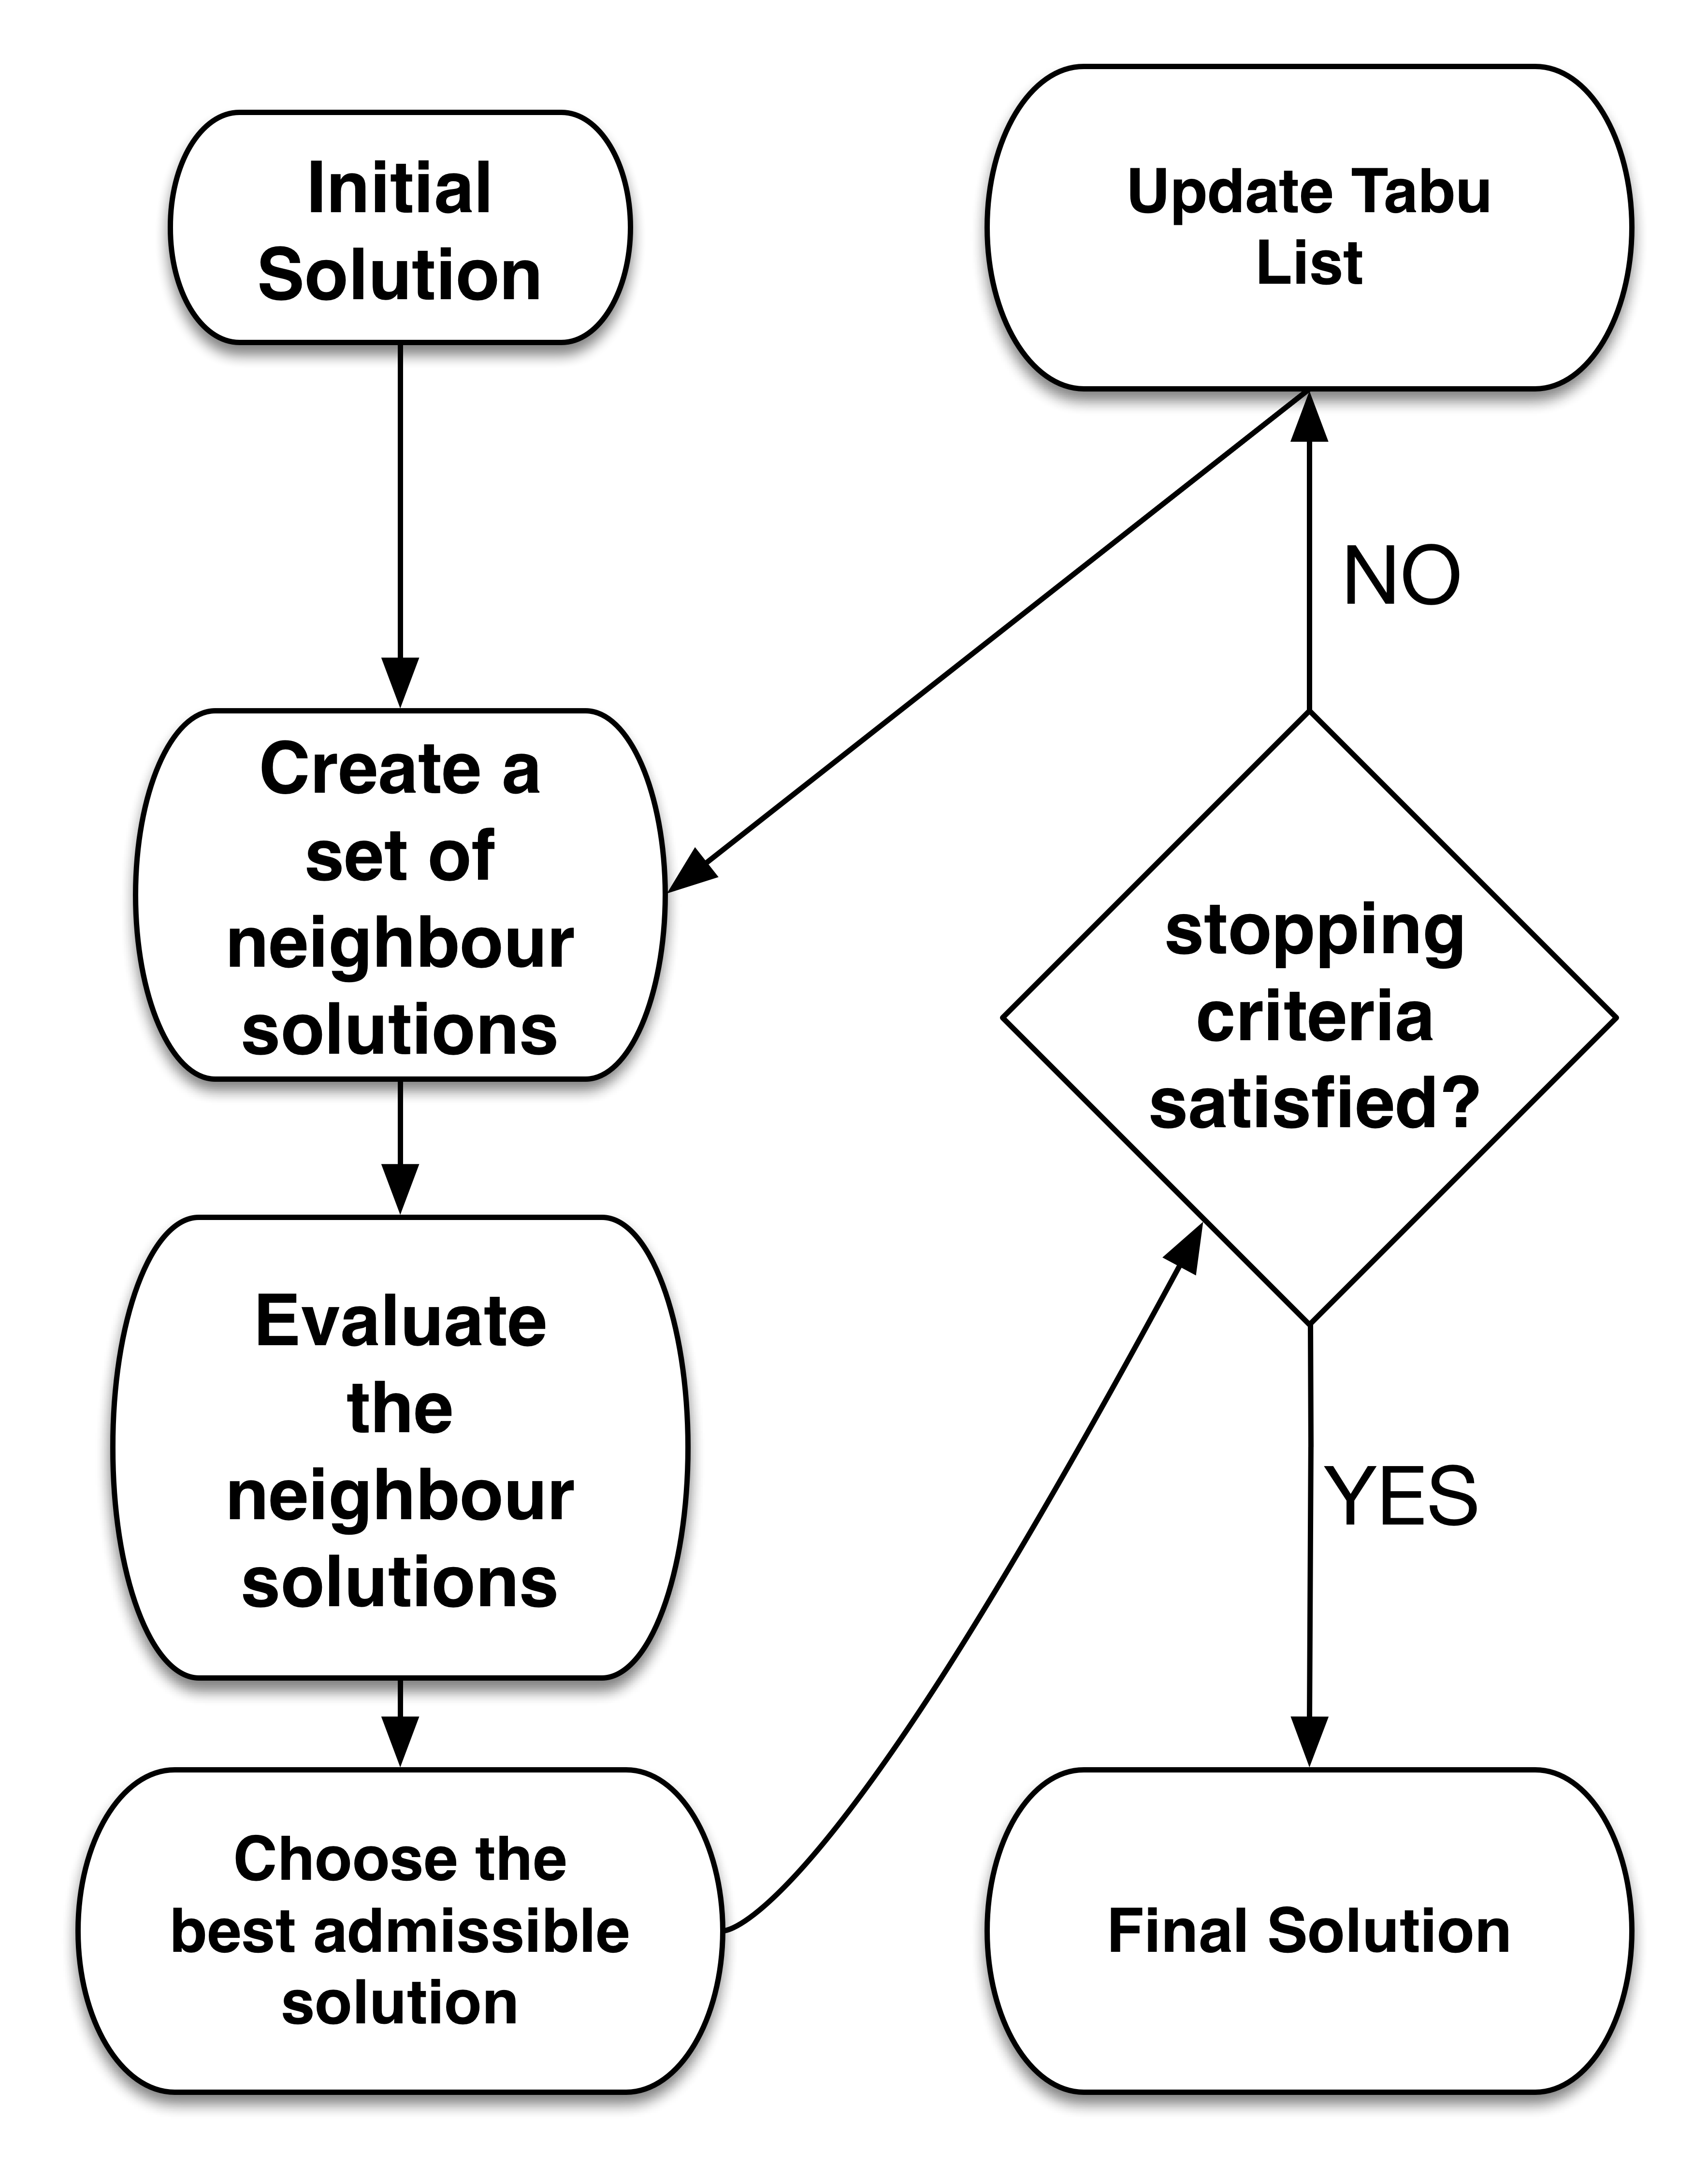
\includegraphics[width=0.4\textwidth]{./images/tabualgorithm.png}
\caption{Tabu Search Algorithm}
\label{fig:tabualg}
\end{figure}


Tabu search  classify a subset of the moves in a neighborhood as forbidden. A tabu list records forbidden moves, which are referred to as tabu moves. A neighborhood is constructed to identify adjacent solutions that can be reached from current solution \cite{reeves1993modern}. 

Tabu restrictions are subject to an important exception.  When a tabu move has a evaluation where it would result in a solution better than any visited so far, then its tabu classification may be overridden.  A condition that allows such an override to occur is called an aspiration criterion \cite{reeves1993modern}. 

The Tabu search uses three main strategies \cite{reeves1993modern}:

\begin{itemize}
\item Forbidding strategy: control what enters the tabu list;
\item Freeing strategy: control what exits the tabu list and when; and
\item Short-term strategy: manage interplay between the forbidding strategy and freeing strategy to select trial solutions.
\end{itemize}